% Created 2017-04-04 Tue 09:36
% Intended LaTeX compiler: pdflatex
\documentclass[11pt]{article}
\usepackage[utf8]{inputenc}
\usepackage[T1]{fontenc}
\usepackage{graphicx}
\usepackage{grffile}
\usepackage{longtable}
\usepackage{wrapfig}
\usepackage{rotating}
\usepackage[normalem]{ulem}
\usepackage{amsmath}
\usepackage{textcomp}
\usepackage{amssymb}
\usepackage{capt-of}
\usepackage{hyperref}
\usepackage[margin=1.2in]{geometry}
\usepackage{setspace}
\onehalfspacing
\usepackage{parskip}
\newcommand{\pr}{\mathrm{Pr}}
\setcounter{secnumdepth}{1}
\author{Zheng Tian}
\date{}
\title{Replication of Examples in Chapter 5}
\hypersetup{
 pdfauthor={Zheng Tian},
 pdftitle={Replication of Examples in Chapter 5},
 pdfkeywords={},
 pdfsubject={},
 pdfcreator={Emacs 25.1.1 (Org mode 9.0.3)},
 pdflang={English}}
\begin{document}

\maketitle

\section{Introduction}
\label{sec:org88266ff}

In this document, I will show you how to perform hypothesis testing
for a single coefficient in a simple linear regression model. I will
do this through replicating the examples that appear in Chapter 5.


\section{The OLS estimation}
\label{sec:org3578b11}

The linear model is
\begin{equation}
\label{eq:testscr-str-1}
TestScore_i = \beta_0 + \beta_1 STR_i + u_i
\end{equation}

We first read data from the Stata file, \texttt{caschool.dta}, into R.
\begin{verbatim}
library(AER)
library(foreign)
classdata <- read.dta("caschool.dta")
\end{verbatim}

Then, we estimate the linear regression model with the function \texttt{lm()}
and get the estimation results using the function \texttt{summary()}.
\begin{verbatim}
df2use <- classdata[c("testscr", "str")]
mod1 <- lm(testscr ~ str, data = df2use)
summary(mod1)
\end{verbatim}

\begin{verbatim}
Call:
lm(formula = testscr ~ str, data = df2use)

Residuals:
    Min      1Q  Median      3Q     Max
-47.727 -14.251   0.483  12.822  48.540

Coefficients:
            Estimate Std. Error t value Pr(>|t|)
(Intercept) 698.9330     9.4675  73.825  < 2e-16 ***
str          -2.2798     0.4798  -4.751 2.78e-06 ***
---
Signif. codes:  0 ‘***’ 0.001 ‘**’ 0.01 ‘*’ 0.05 ‘.’ 0.1 ‘ ’ 1

Residual standard error: 18.58 on 418 degrees of freedom
Multiple R-squared:  0.05124,	Adjusted R-squared:  0.04897
F-statistic: 22.58 on 1 and 418 DF,  p-value: 2.783e-06
\end{verbatim}


The estimation results reported by \texttt{summary(mod1)} include the
estimated coefficients, their standard errors, t-statistics, and the
p-values. There are other statistics that we will learn in the next
two lectures.

By default, the standard errors reported are computed using
the formula of \textbf{the homoskedasticity-only standard errors}, which are
then used to compute the t-statistics. And the p-values are based on
the Student's t distribution with 418 degrees of freedom.


\section{Hypothesis tests}
\label{sec:orgbf56b7b}

Now we get into testing the hypothesis regarding \(\beta_1\), that is,
\[ H_0: \beta_1 = \beta_{1,0} \text{ vs. } H_1: \beta_1 \neq
\beta_{1,0} \]

In this example, we are testing the null hypothesis \(H_0: \beta_1 =
0\).

\subsection*{Compute the t-statistic}
\label{sec:org80a95a5}

We compute the t-statistic based on the
following formula,

\begin{equation}
\label{eq:t-stat-b1}
t = \frac{\hat{\beta}_1 - \beta_{1,0}}{SE(\hat{\beta}_1)}
\end{equation}

Upon computing the t-statistic, we compare it with the critical value
at the desired significant level, say 5\%, which is 1.96 for a
two-sided test with the standard normal distribution. Also, we can use
the t-statistic to get the p-value.

How can we get all the quantities used in this formula? Of course, you
can simply copy them from the output of \texttt{summary(mod1)}. But doing so
is cumbersome and prone to mistakes. More importantly, we should use
the \textbf{heteroskedasticity-robust standard error} of \(\hat{\beta}_1\)
instead of the ones reported by default.

Next, I will show you two ways to get the t-statistics using the
heteroskedasticity-robust standard errors. The first way is to get all
the quantities in Equation (\ref{eq:t-stat-b1}) using R
functions, and the second way is to get the appropriate t-statistic
through the function \texttt{coeftest()}. Although the second method is much
easier than the first one, we can learn how to obtain all the elements
in the output of the function \texttt{lm()}.


\subsection*{Get all elements from an \texttt{lm} object}
\label{sec:orgd78f922}

\subsubsection*{The coefficients}
\label{sec:org014a1e2}

The output of the function \texttt{lm()} is an \texttt{lm} object that has the same
structure as a \texttt{list} object.
\begin{verbatim}
class(mod1)
str(mod1, max.level=1, give.attr = FALSE)
\end{verbatim}

\begin{verbatim}
[1] "lm"
List of 12
 $ coefficients : Named num [1:2] 698.93 -2.28
 $ residuals    : Named num [1:420] 32.7 11.3 -12.7 -11.7 -15.5 ...
 $ effects      : Named num [1:420] -13406.2 88.3 -14 -12.6 -16.8 ...
 $ rank         : int 2
 $ fitted.values: Named num [1:420] 658 650 656 659 656 ...
 $ assign       : int [1:2] 0 1
 $ qr           :List of 5
 $ df.residual  : int 418
 $ xlevels      : Named list()
 $ call         : language lm(formula = testscr ~ str, data = df2use)
 $ terms        :Classes 'terms', 'formula'  language testscr ~ str
 $ model        :'data.frame':	420 obs. of  2 variables:
\end{verbatim}

From an \texttt{lm()} object, all estimated coefficients can be extracted
using the function \texttt{coef()}, which returns a vector containing all
estimated coefficients. By default, the first element in the vector is
the estimated intercept, and the slope is the second.

\begin{verbatim}
b <- coef(mod1)
b
\end{verbatim}

\begin{verbatim}
(Intercept)         str
 698.932952   -2.279808
\end{verbatim}

\begin{verbatim}
b1 <- b[2]
\end{verbatim}

\subsubsection*{The standard errors}
\label{sec:orgdcad95a}

\begin{itemize}
\item The homoskedasticity-only standard errors are reported in the output
of \texttt{summary()} by default in R. They can also be extracted with the
function, \texttt{vcov()}, which returns a matrix called the covariance
matrix, with the diagonal elements representing the variances of the
estimated coefficients. Thus, the standard errors are the square
roots of the diagonal elements.

\begin{verbatim}
V <- vcov(mod1)
se_b1 <- sqrt(V[2, 2]); se_b1
\end{verbatim}

\begin{verbatim}
[1] 0.4798256
\end{verbatim}

\item The heteroskedasticity-robust standard errors are the square roots
of the diagonal elements in the \textbf{heteroskedasticity-consistent}
covariance matrix, obtained using the function of \texttt{vcovHC()} in
the \texttt{sandwich} package that is loaded by default. There are several
versions of the heteroskedasticity-consistent covariance
matrix. What we use is the type of \texttt{HC1}.

\begin{verbatim}
htV <- vcovHC(mod1, type = "HC1")
se_b1_rb <- sqrt(htV[2, 2]); se_b1_rb
\end{verbatim}

\begin{verbatim}
[1] 0.5194892
\end{verbatim}
\end{itemize}

\subsubsection*{The t-statistic, the critical value, and the p-value}
\label{sec:org7298d2d}

The t-statistics using the heteroskedasticity-robust standard error
is then computed by
\begin{verbatim}
(t_b1_rb <- b1 / se_b1_rb)
\end{verbatim}

\begin{verbatim}
      str
-4.388557
\end{verbatim}

Although we know the critical value at the 5\% significant level for a
two-sided test is 1.96 with a large sample, we prefer getting the
value from a function in R. The critical value at the 5\% significance
level is in fact the 97.5\(^{\text{th}}\) percentile of the standard normal
distribution, which can be obtained from the \texttt{qnorm()} function.

\begin{verbatim}
(c.5 <- qnorm(0.975))
\end{verbatim}

\begin{verbatim}
[1] 1.959964
\end{verbatim}

The p-value associated with the actual t-statistics is
\(\mathrm{Pr}\left(|t| > |t^{act}| \right) = 2 \Phi(-|t^{act}|)\). We can
compute the p-value in R, following this definition and using the
\texttt{pnorm()} function.

\begin{verbatim}
(pval <- 2 * pnorm(-abs(t_b1_rb)))
\end{verbatim}

\begin{verbatim}
         str
1.141051e-05
\end{verbatim}


\subsection*{Use \texttt{coeftest()}}
\label{sec:orga2838d3}

Since hypothesis testing is a very common work in statistics, many R
functions have been developed to do it. Here I introduce a function,
\texttt{coeftest()}, which is in the package of \texttt{lmtest} loaded automatically
through loading the \texttt{AER} package.

\begin{verbatim}
coeftest(mod1)
\end{verbatim}

\begin{verbatim}

t test of coefficients:

             Estimate Std. Error t value  Pr(>|t|)
(Intercept) 698.93295    9.46749 73.8245 < 2.2e-16 ***
str          -2.27981    0.47983 -4.7513 2.783e-06 ***
---
Signif. codes:  0 ‘***’ 0.001 ‘**’ 0.01 ‘*’ 0.05 ‘.’ 0.1 ‘ ’ 1
\end{verbatim}

By default, it reports the homoskedasticity-only standard errors,
the corresponding t-statistics, and the p-values. To get the
heteroskedasticity-robust results, we need to add an argument to this
function to specify the heteroskedasticity-consistent covariance
matrix, which has been defined above as \texttt{htV <- vcovHC(mod1, type = "HC1")}.

\begin{verbatim}
# coeftest returns a matrix
t_tst <- coeftest(mod1, vcov. = htV); t_tst
\end{verbatim}

\begin{verbatim}

t test of coefficients:

             Estimate Std. Error t value  Pr(>|t|)
(Intercept) 698.93295   10.36436 67.4362 < 2.2e-16 ***
str          -2.27981    0.51949 -4.3886 1.447e-05 ***
---
Signif. codes:  0 ‘***’ 0.001 ‘**’ 0.01 ‘*’ 0.05 ‘.’ 0.1 ‘ ’ 1
\end{verbatim}

\begin{verbatim}
## Get the t-statistic for STR
t_b1 <- t_tst["str", "t value"]; t_b1
\end{verbatim}

\begin{verbatim}
[1] -4.388557
\end{verbatim}


\subsection*{Confidence interval}
\label{sec:org136b84d}

Finally, we can construct the 95\% confidence interval of \(\beta_1\)
using the function of \texttt{confint()}, which uses the
homoskedasticity-only standard errors.
\begin{verbatim}
# confidence interval with the default homoskedasticity-only SE
confint(mod1, "str")
\end{verbatim}

\begin{verbatim}
       2.5 %    97.5 %
str -3.22298 -1.336637
\end{verbatim}

Since there is no existing function to report the confidence interval
with heteroskedasticity-robust SE, we can write a user-defined
function to do that.

\begin{verbatim}
get_confint_rb <- function(lm_obj, param, vcov_ = vcov(lm_obj),
			   level = 0.05){
    ## This function generates a two-sided confidence interval for a
    ## parameter in the linear regression model with a specified
    ## covariance matrix.  The inputs The output

    ## get all the parameters' names and select one based on param
    all_param <- names(coef(lm_obj))
    which_param <- grep(param, all_param)

    ## get the estimated parameter and its standard error
    bhat_param <- coef(lm_obj)[which_param]
    sd_param <- sqrt(vcov_[which_param, which_param])

    ## get the critical value
    cv <- qnorm(1 - level/2)

    ## calculate the confidence interval
    lower <- bhat_param - cv * sd_param
    upper <- bhat_param + cv * sd_param

    conf_interval <- c(lower, upper)
    names(conf_interval) <- c("lower", "upper")
    return(conf_interval)
}
\end{verbatim}

Note that we define the default value of \texttt{vcov\_} to be the
homoskedasticity-only covariance matrix in the function
\texttt{get\_confint\_rb()}, and the default significant level is 5\%. When
computing the confidence interval with the heteroskedasticity-robust
standard errors, we need to change \texttt{vcov\_} to a
heteroskedasticity-consistent covariance matrix, which is \texttt{htV}.

\begin{verbatim}
get_confint_rb(mod1, param = "str", vcov = htV)
\end{verbatim}

\begin{verbatim}
    lower     upper
-3.297988 -1.261628
\end{verbatim}


\section{Dummy variable}
\label{sec:org1abefc0}

\subsection*{Create a dummy variable}
\label{sec:orgc20ccf8}

We define a dummy variable representing small classes.
\begin{equation*}
D_i =
\begin{cases}
1,\; &\text{ if } str < 20 \\
0,\; &\text{ if } str \geq 20
\end{cases}
\end{equation*}

\begin{verbatim}
smallclass <- ifelse(df2use$str < 20, 1, 0)
\end{verbatim}

The function \texttt{ifelse()} creates a vector consisting of 1 and 0. The
first argument in this function is a condition, \texttt{df2use\$str < 20}. If the
condition is satisfied for an element in \texttt{df2use\$str}, the corresponding
element in \texttt{D} is 1, otherwise 0.


\subsection*{Regression with a dummy variable}
\label{sec:org95594d2}

Then we can estimate the linear regression of test scores against the
dummy variable, and do the zero hypothesis test.

\begin{verbatim}
mod2 <- lm(testscr ~ smallclass, data = df2use)
coeftest(mod2, vcov. = vcovHC(mod2, type = "HC1"))
\end{verbatim}

\begin{verbatim}

t test of coefficients:

            Estimate Std. Error  t value  Pr(>|t|)
(Intercept) 649.9788     1.3229 491.3317 < 2.2e-16 ***
smallclass    7.3724     1.8236   4.0428 6.288e-05 ***
---
Signif. codes:  0 ‘***’ 0.001 ‘**’ 0.01 ‘*’ 0.05 ‘.’ 0.1 ‘ ’ 1
\end{verbatim}


\subsection*{Create a scatterplot}
\label{sec:orgfcd5ef1}

We can create a scatterplot to visualize the relationship between test
scores and the dummy variable.
\begin{verbatim}
plot(smallclass, df2use$testscr,
     xlab = "class size", ylab = "test score")
\end{verbatim}

\begin{figure}[htbp]
\centering
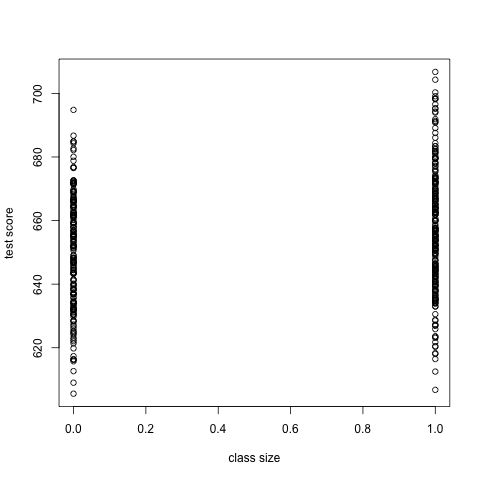
\includegraphics[width=0.8\textwidth]{scatter_smallclass.png}
\caption{\label{fig:orgd00e814}
The scatterplot without jittering}
\end{figure}

In Figure \ref{fig:orgd00e814}, since the variable \texttt{smallclass} takes only
the value of 1 or 0, many points are overlapped. To make these points
more visible, we can create a scatterplot with jittered points. I also
adjust the limit of x-axis so that the clusters of points appear close
towards the center of the plot.

\begin{verbatim}
smallclass_jittered <- jitter(smallclass, amount = 0.05)
plot(smallclass_jittered, df2use$testscr, xlim = c(-0.5, 1.5),
     xlab = "class size", ylab = "test score")
abline(coef(mod2)[1], coef(mod2)[2], col = "blue")
\end{verbatim}

\begin{figure}[htbp]
\centering
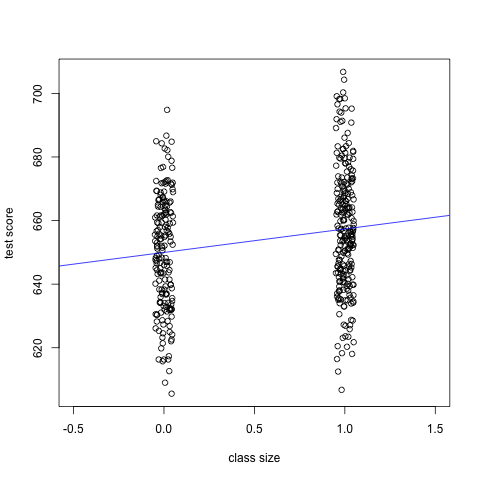
\includegraphics[width=0.8\textwidth]{jittered_scatter_smallclass.png}
\caption{\label{fig:orgf47fd2e}
The scatterplot with jittering}
\end{figure}
\end{document}